% -*- mode: latex; mode: auto-fill; coding: utf-8; -*-

\chapter{Test Data}
\label{chapter:test_data}
% This section describes the meshes and material properties we have been
% testing our simulator with.

\section{Materials}
\label{sec:test-materials}

Table \vref{table:test-materials} lists the material properties that
were used during testing. The material properties are measured at room
temperature and at 1013.25 hPa (1 atm) pressure.

\begin{table}
  \centering
  \begin{tabular}{| l | r | r | r | r | r |}
    \hline
    name     & $E$ & $\nu$ & $\rho$   & $\sigma_F^+$ & $\sigma_F^-$ \\
    unit     & GPa &       & $kg/m^3$ & MPa          & MPa \\
    \hline
    concrete &  41 &  0.21 &     2400 &            5 & 40 \\

%    cement    &  11.2 &       & 0.21 & 2010 & 0.91 &  ? \\
%    ceramic   &   400 &     ? &    ? & 3000 &    ? &  ? \\
%    glass     &    71 &    30 &      & 2450 & 3500 &  ? \\
%    steel     &   210 &    80 &  0.3 & 7850 &    ? &  ? \\
%    iron (FE) &     ? &     ? &    ? &    ? & 7870 &  ? \\
%    rubber    & 0.004 & 0.001 &  0.5 & 1000 &    ? &  ? \\
%    porcelain &    60 &     ? &    ? &    ? &   50 & 250 \\
     dentin & 12 &     0.32 & 2580 &  100 & 250 \\
%    email     &    50 &     ? &    ? &    ? &   10 & 250 \\
    \hline
  \end{tabular}
  \caption{Data for test materials.}
  \label{table:test-materials}
\end{table}

When $E$ is the elasticity modulus, $\nu$ is Poisson's ratio, $\rho$
the density, $\sigma_F^+$ the tensile strength, and $\sigma_F^-$ the
compressive strength. The data for concrete was found on the
web\footnote{\url{http://www.engineeringtoolbox.com/concrete-properties-d_1223.html}}.
The data for dentin was found in the following references:
$\nu = 0.32$ \citebook{page~19}{article:dentin-material},
$\rho = 2580 kg/m^3$ \citebook{page~25}{book:dentist-materials},
$E = 12 GPa$ \citebook{page~29}{book:dentist-materials},
$\sigma_F^+ = 100 GPa$, and $\sigma_F^- = 250 GPa$
\citebook{page~71}{book:leas}.

\section{The Meshes}
We have three different kind of objects that we want to test.
%
The first kind are simple objects, these objects are small models that
can be used to produce a minimal amount of output data, which makes
analysis easier.
%
The second object kind is called a bar, which is a rectangular object with
dimensions $160mm \times 40mm \times 20mm$.
%
The third kind of objects are teeth. These are tightly coupled to the
surgical scenario that we are trying to simulate.

\layoutnewpage

\subsection{The simple objects}
Table \vref{table:simple-meshes} described the simple objects we have
been using.

\begin{table}
  \centering
  \begin{tabular}{| l | r | r | r |}
    \hline
    name & \# nodes & \# surface triangles & \# body tetrahedra \\
    \hline
    tetrahedron & 4 & 4 & 1 \\
    box & 14 & 24 & 17 \\
    sphere & 119 & 212 & 328 \\
    \hline
  \end{tabular}
  \caption{Data for the simple meshes.}
  \label{table:simple-meshes}
\end{table}

\subsection{The Bar Object}
\label{sec:bar-mesh}
To model the bar object, we have four meshes with different resolutions.
%
The models have been constructed using the Blender modelling tool,
which is a tool for constructing surfaces meshes. The models have been
constructed as quadratic surface elements in Blender by subdividing
the bar as shown in figure \vref{fig:blender-bars} for the four meshes.

\begin{figure}
  \centering
  \subfloat[bar $20 \times 20 \times 20$.]{
    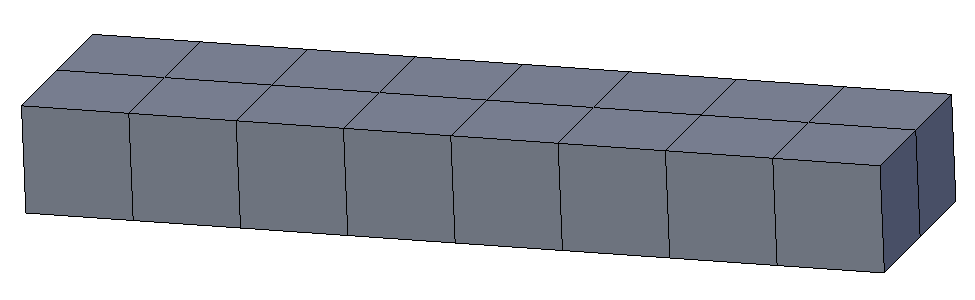
\includegraphics[width=7cm]{./images/appendix_test_data_bar_20.png}
    \label{fig:bar20}
  }
  \subfloat[bar $10 \times 10 \times 10$.]{
    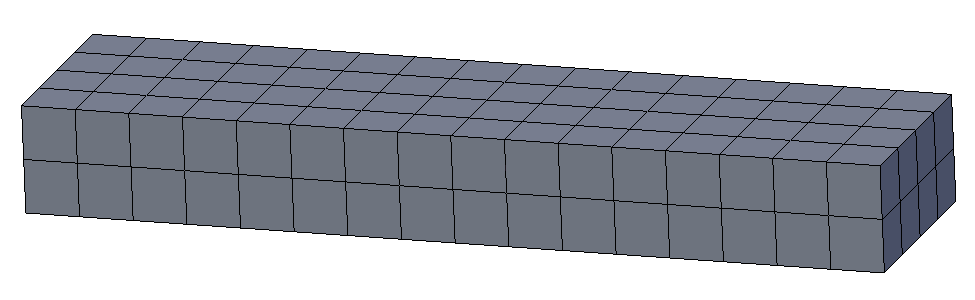
\includegraphics[width=7cm]{./images/appendix_test_data_bar_10.png}
    \label{fig:bar10}
  }
  \newline
  \subfloat[bar $5 \times 5 \times 5$.]{
    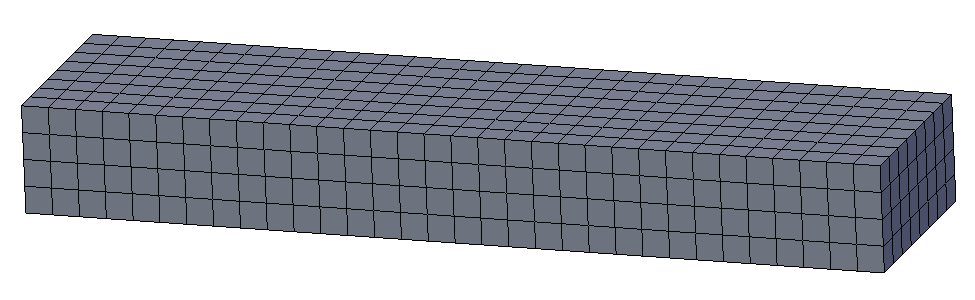
\includegraphics[width=7cm]{./images/appendix_test_data_bar_5.png}
    \label{fig:bar5}
  }
  \subfloat[bar $2.5 \times 2.5 \times 2.5$.]{
    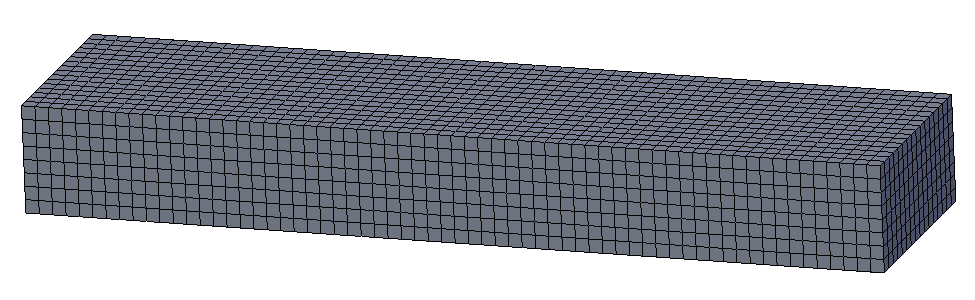
\includegraphics[width=7cm]{./images/appendix_test_data_bar_2_5.png}
    \label{fig:bar2-5}
  }
  \caption{The four different bar resolutions.}
  \label{fig:blender-bars}
\end{figure}

Afterwards the quadratic meshes have been automatically triangularized
by Blender. Then the surface meshes must be converted into a
volumetric mesh via TetGen, the whole process is described in appendix
\appref{sec:constructing-meshes}. The final stats of the four meshes can
be seen in table \vref{table:bar-meshes}.

\begin{table}
  \centering
  \begin{tabular}{| l | r | r | r |}
    \hline
    name & \# nodes & \# surface triangles & \# body tetrahedra \\
    \hline
    bar $20 \times 20 \times 20$ & 113 & 210 & 263 \\
    bar $10 \times 10 \times 10$ & 373 & 708 & 964\\
    bar $5 \times 5 \times 5$ & 1619 & 3004 & 4658 \\
    bar $2.5 \times 2.5 \times 2.5$ & 6297 & 10214 & 21809 \\
    \hline
  \end{tabular}
  \caption{Data for the different bar resolutions.}
  \label{table:bar-meshes}
\end{table}

\layoutnewpage

\subsection{The Tooth Object}
\label{sec:test-data-tooth}
The tooth object is modeled with a few different kinds of meshes
depending on in which kind of scenario we are using it. Basicly we
have two models, a test tooth and a model of a real wisdom tooth. The test
tooth is a rectangular model like the bar, but this model has a slice
50\% through the middle of the object. The test tooth is illustrated
in figure \vref{fig:test-tooth-side}. The real tooth object comes in
two variants, one with a slice 33\% through the body, modelling a
drill hole, and another without the slice. These two can be seen in
figure \ref{table:tooth-meshes} and \vref{fig:tooth-side}
respectively. We also have these two variants in different
resolutions, the original model and a simplified version. The simple
version has been generated using the Quadric Edge Collapse Decimation
tool in MeshLab.

\begin{figure}
  \centering
  \subfloat[Tooth from the front.]{
    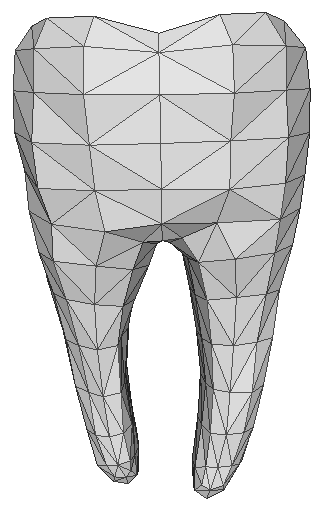
\includegraphics[width=7cm]{./images/appendix_test_data_tooth_wf_front.png}
    \label{fig:tooth-front}
  }
  \subfloat[Tooth above.]{
    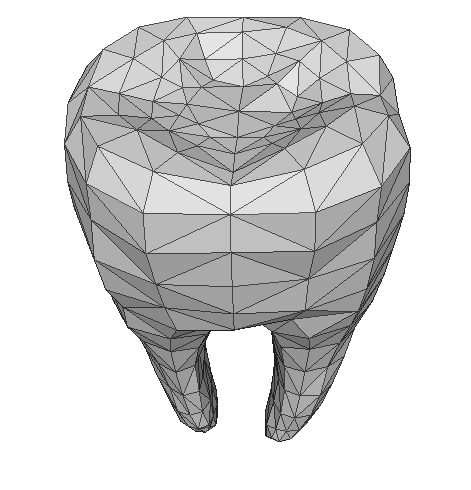
\includegraphics[width=8cm]{./images/appendix_test_data_tooth_wf_above.png}
    \label{fig:tooth-above}
  }
  \caption{The tooth test model.}
  \label{fig:tooth-noslice}
\end{figure}

\layoutnewpage

\begin{figure}
  \centering
  \subfloat[Tooth with 33\% slice.]{
    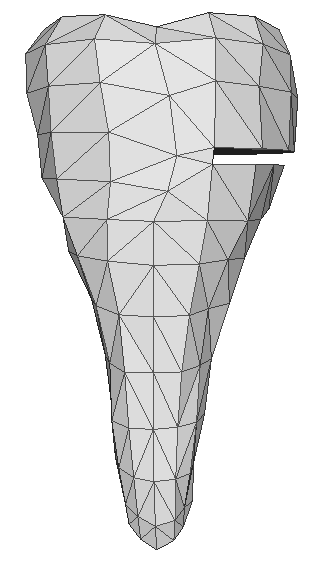
\includegraphics[width=5cm]{./images/appendix_test_data_tooth_wf_side.png}
    \label{fig:tooth-side}
  }
  \subfloat[Test tooth with 50\% slice.]{
    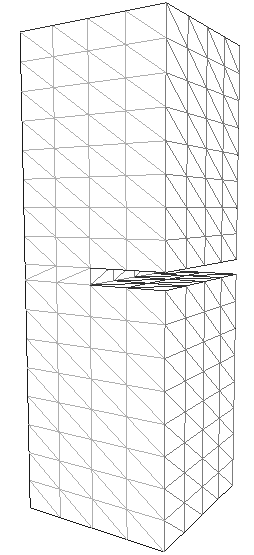
\includegraphics[width=4cm]{./images/appendix_test_data_test_tooth_wf.png}
    \label{fig:test-tooth-side}
  }

  \subfloat[Closeup of the drill hole in tooth with 33\% slice.]{
    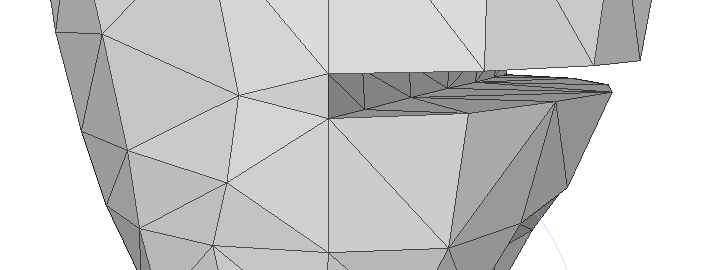
\includegraphics[width=7cm]{./images/appendix_test_data_tooth_wf_closeup.png}
    \label{fig:tooth-closeup}
  }
  \caption{Tooth models with slice.}
  \label{fig:tooth-slice}
\end{figure}

The stats for the tooth models are described in table
\vref{table:tooth-meshes}.

\begin{table}
  \centering
  \begin{tabular}{| l | r | r | r |}
    \hline
    name & \# nodes & \# surface triangles & \# body tetrahedra \\
    \hline
    tooth & 667 & 1100 & 2264 \\ 
    tooth with 33\% slice & 748 & 1198 & 2677 \\ 
    tooth (simple)                  & 371 & 680 & 1168   \\
    tooth with 33\% slice (simple)  & 483 & 826 &  1652  \\
    test tooth with 50\% slice & 646 & 1180 & 1902 \\
    test tooth high resolution with 50\% slice & 2763 & 4808 & 8819 \\
    \hline
  \end{tabular}
  \caption{Data for the different tooth meshes.}
  \label{table:tooth-meshes}
\end{table}

